\documentclass[12pt]{report}
\usepackage[a4paper, left=3.17cm, right=3.17cm, top=2.54cm, bottom=2.54cm]{geometry}
\usepackage[T1]{fontenc}
\usepackage{mathptmx}
\usepackage{amsmath}
\usepackage{amsfonts}
\usepackage{chemformula}
\usepackage{multicol}
\usepackage{multirow}
\usepackage{tabularx,booktabs}
\newcolumntype{C}{>{\centering\arraybackslash}X} % centered version of "X" type
\usepackage[linesnumbered,ruled,vlined]{algorithm2e}
\usepackage{comment}
\usepackage{array}
\newcolumntype{P}[1]{>{\centering\arraybackslash}p{#1}}
\usepackage{cite}
\usepackage[colorlinks, linkcolor=black, anchorcolor=black, citecolor=black]{hyperref}
\usepackage{graphicx}
\setlength{\parskip}{0.5em}
\title{Employee Management System}
%\author{\textup{Qi YUAN}}


% Assembly Code Start
\usepackage{listings}
\usepackage{xcolor} % Optional: For syntax highlighting

\lstset{
    basicstyle=\ttfamily\small,       % Use monospace font for code
    keywordstyle=\color{blue},        % Set keywords to blue
    commentstyle=\color{green!60!black}, % Set comments to green
    stringstyle=\color{violet},          % Set strings to red
    numbers=left,                     % Display line numbers on the left
    numberstyle=\tiny,                % Line number font size
    stepnumber=1,                     % Line number increment
    breaklines=true,                  % Enable line wrapping
    frame=single,                     % Add a frame around the code
    captionpos=b,                     % Caption position (below code)
    xleftmargin=10pt,                 % Left margin for the code block
    tabsize=4,                        % Set tab width
    showstringspaces=false            % Hide spaces in strings
}

% Assembly Code End


%copyright at footer
\usepackage{fancyhdr}
\fancyhf{}
\rfoot{%
  \footnotesize
  \textcopyright~Dept. of Computer Science and Engineering, GUB\\

 }
%\pagestyle{fancy}


\begin{document}
    \input{title/title.tex}
    \tableofcontents
  


% Chapter 1 starting here.....    
\newpage
\chapter{Introduction}

\section{Overview}
\includecomment{Start the section with a general discussion of the project, that is, an overview.}
The Employee Management System (EMS) is an 8086 assembly project designed to manage employee data within an organization. The system features an authentication step to ensure secure and personalized access. This program handles basic tasks such as adding new employee information, deleting the last added employee information, and showing all existing employee information. In addition, the user can log out and exit the program from the main menu.

\section{Motivation}
\includecomment{Write this section mentioning actually why you have decided to choose this project.}
The motivation behind this project is to test the capabilities of the 8086 assembly program. This program shows the data storage and handling capabilities of the 8086 assembly language. 

\section{Problem Definition}

\subsection{Problem Statement}
\includecomment{Here you will describe the the statement that you want to address as your problem. This will definitely contain discussion according to your above motivation.}

Higher-level languages make storing and managing employee information much easier, and user interfaces can be easily developed using them. However, in lower-level languages like assembly, these simple tasks become significantly more challenging.

\subsection{Complex Engineering Problem}
\includecomment{The following table must be completed according to your above discussion in detail. The column on the right side should be filled only on the attributes you have chosen to be touched by your own project.}

The biggest challenge in this project is to securely store employee information and create a simple and user-friendly interface.


\begin{table}[htbp]
   \centering
    \caption{Summary of the attributes touched by the mentioned projects}
    \begin{tabular}{|p{6.0 cm}|p{8 cm}|}
    %\rowcolor{gray!30}
    \toprule
        \textbf{Name of the P Attributes} & \textbf{Explain how to address}  \\
        \midrule

    \textbf{P1:} Depth of knowledge required  &  In depth knowledge of registers and assembly language is required.\\
      \hline
       
    \textbf{P2:} Range of conflicting
     requirements  &  ---- \\
      \hline

    \textbf{P3:} Depth of analysis required  &  Analysis about registers is required.\\
    \hline
    
    \textbf{P4:} Familiarity of issues  &  ---- \\ 
    \hline
    \textbf{P5:} Extent of applicable codes  &  ---- \\
      \hline
       
    \textbf{P6:} Extent of stakeholder
     involvement and conflicting
     requirements  &  ---- \\
      \hline

    \textbf{P7:} Interdependence  &  You need to consider the interdependence of the program with other systems and platforms, such as the campus network, compatibility on different platforms, such as linux and windows. \\
    \hline
        
    \end{tabular}
    \label{tab:IC}
\end{table}

\section{Design Goals/Objectives}
\includecomment{Specify and discuss the goals or objectives of your project.}

The primary objectives of this project are:
\begin{itemize}
    \item Implement user authentication using username and password.
    \item Create a user-friendly interface to navigate through the program.
    \item Implement basic features such as add, delete, and show all employee information.
    \item Efficiently store the employee information.
    \item Test the capabilities of the 8086 assembly program.
 
 
 
 
\end{itemize}


\subsection{Application}
\subsubsection{Efficient Employee Data Management}
The EMS simplifies storing, organizing, and managing employee data.
\subsubsection{Attendance Tracking}
Keep track of employee attendance records, including clock-in/out times, leave requests, 
and absences.
\subsubsection{Payroll Management}
Calculate salaries, deductions, and bonuses. Handle tax calculations and generate pay stubs.
\subsubsection{Quick and Accurate Information Retrieval}
The system’s search functionality allows administrators to quickly retrieve specific 
employee information.
\begin{comment}

\section{Application}
\includecomment{Write about the exact application of your chosen project in the real world in details.In every section please add subsections and figures and citations as references also.}

The employee management system project has many real-world applications such as, data management in various organizations, storing and managing employee information to easily manage human resource, keeping track of all employee information, etc. This system can be implemented in any management system application.

    

\section{Tools}

\textbf{EMU8086:} The emu8086  microprocessor emulator is a free emulator for multiple platforms. It provides its user with the ability to emulate old 8086 processors. 


% Chapter 1 ends here.....    


% Chapter 2 starting here.....    
\newpage
\chapter{Design/Development/Implementation of the Project}

\section{Introduction}
\includecomment{Start the section with a general discussion of the project }

The employee management system is a simple application that helps the organization keep track of the employee information, such as their names, IDs, contact details, etc. It aims to develop a user-friendly interface and provide basic functionalities using 8086 assembly language.

\section{Project Details}

\subsection{Login Module}
\begin{itemize}
    \item Validates username and password.
    \item Displays success or error messages based on input.
\end{itemize}

\subsection{Main Menu}
\begin{itemize}
    \item Lists options to add, delete, show all employee information etc.
    \item Each option has unique key and user-interface.
\end{itemize}

\subsection{Add Employee}
\begin{itemize}
    \item Add new employee name, email and phone.
    \item Show success or error message.
\end{itemize}

\subsection{Delete Employee}
\begin{itemize}
    \item Delete the last added employee information.
    \item Show success or error message.
\end{itemize}

\subsection{Show All Employee}
\begin{itemize}
    \item List all employee information in a table format.
\end{itemize}

\subsection{Logout and Exit Program}
\begin{itemize}
    \item Logout and return to admin login page.
    \item Press designated key to exit the program.
\end{itemize}


\section{Implementation}
\includecomment{All the implementation details of your project should be included in this section, along with many subsections.}


\subsection{Source Code}

\lstset{language=[x86masm]Assembler} % Set the language for highlighting
\begin{lstlisting}

include 'emu8086.inc'
.model small
.stack 100h
.data
    ; Utilities
    newLine          db 10, 13, "$" ; Newline

    ; Login Page
    l1 db 13, 10, "**************************************************$" 
    l2 db 13, 10, "**                  Admin Login                 **$" 
    l3 db 13, 10, "**************************************************$" 

    askUsername db "Enter Username: $" 
    askPassword db "Enter Password: $" 

    loginSuccessMsg db "Login Successful! $" 
    loginErrorMsg db "Login Failed! (Press Any Key to Continue) $"

    username db "admin" ; Predefined username
    password db "admin" ; Predefined password

    inUsername db 10 dup("$") ; Buffer for input username (10 characters max)
    inPassword db 10 dup("$") ; Buffer for input password (10 characters max)

    ; Main Menu
    m1 db 13, 10, "**************************************************$" 
    m2 db 13, 10, "**                   Employee                   **$" 
    m3 db 13, 10, "**                  Management                  **$" 
    m4 db 13, 10, "**                    System                    **$" 
    m5 db 13, 10, "**************************************************$"

    ; Main Menu Options
    mmOption1        db 13, 10, "1. Add Employee $"
    mmOption2        db 13, 10, "2. Delete Last Added Employee $"
    mmOption3        db 13, 10, "3. Show All Employees $"
    mmOption4        db 13, 10, "4. Logout $"
    mmOption5        db 13, 10, "5. Exit Program $"
    mmChoice         db 13, 10, "Enter Your Choice: $"

    ; Employee Data Storage
    empCount         db 0                       ; Count of employees added
    empNames         db 10 dup(30 dup('$'))     ; Storage for 10 employee names, each 30 characters max
    empEmails        db 10 dup(30 dup('$'))     ; Storage for 10 employee emails, each 30 characters max
    empPhones        db 10 dup(30 dup('$'))     ; Storage for 10 employee phones, each 30 characters max

    askEmployeeName  db 10, 13, "Name: $"
    askEmployeeEmail db 10, 13, "Email: $"
    askEmployeePhone db 10, 13, "Phone: $"

    deleteSuccessMsg db 10, 13, "Employee deleted successfully!$"
    invalidSerialMsg db "Invalid Serial Number!$"
    noEmployeesDelMsg   db "No employees to delete.$"
    noEmployeesShowMsg   db "No employees to show.$"
    employeeHeader   db "Employee List:$"
    
    tab              db "    |    $"

    ; Add Page
    a1 db 13, 10, "**************************************************$" 
    a2 db 13, 10, "**                  Add Employee                **$" 
    a3 db 13, 10, "**************************************************$"

    ; Delete Page
    d1 db 13, 10, "**************************************************$" 
    d2 db 13, 10, "**                Delete Employee               **$" 
    d3 db 13, 10, "**************************************************$"
    
    ; Show All Page
    s1 db 13, 10, "**************************************************$" 
    s2 db 13, 10, "**                 Employee List                **$" 
    s3 db 13, 10, "**************************************************$"
    
.code
main proc
    mov   ax, @data
    mov   ds, ax

    call DisplayLoginPage
    call ValidateLogin       
    call  DisplayMainMenu
main endp

;-------------------------------------------------

DisplayLoginPage proc
    ; Display login page header
    mov ah, 9
    lea dx, l1
    int 21h
    lea dx, l2
    int 21h
    lea dx, l3
    int 21h
    lea dx, newLine
    int 21h

    print 'Enter Username: '

    ; Get username input from user
    mov si, offset inUsername
InputUsername:
    mov ah, 1
    int 21h
    cmp al, 13      ; Comapare with Enter key
    je DoneUsername
    mov [si], al
    inc si
    jmp InputUsername
DoneUsername:

    ; Prompt for password
    mov ah, 9
    lea dx, newLine
    int 21h
    
    print 'Enter Password: '

    ; Get password input from user
    mov si, offset inPassword
InputPassword:
    mov ah, 1
    int 21h
    cmp al, 13
    je DonePassword
    mov [si], al
    inc si
    jmp InputPassword
DonePassword:
    ret
DisplayLoginPage endp

;-------------------------------------------------

ValidateLogin proc
    ; Validate username
    mov si, offset username
    mov di, offset inUsername
    mov cx, 5
LoginValidationUsername:
    mov bl, [si]
    mov dl, [di]
    cmp bl, dl
    jne InvalidLogin
    inc si
    inc di
    loop LoginValidationUsername

    ; Validate password
    mov si, offset password
    mov di, offset inPassword
    mov cx, 5
LoginValidationPassword:
    mov bl, [si]
    mov dl, [di]
    cmp bl, dl
    jne InvalidLogin
    inc si
    inc di
    loop LoginValidationPassword

    ; Display success message
    mov ah, 9
    lea dx, newLine
    int 21h
    lea dx, newLine
    int 21h
    
    print 'Login Successful!'
    ret

InvalidLogin:
    ; Display error message
    mov ah, 9
    lea dx, newLine
    int 21h

    print 'Login Failed! (Press Any Key to Continue)'

    ; Wait for key press
    mov ah, 1
    int 21h
    jmp main
ValidateLogin endp

;-------------------------------------------------

Logout proc
    ; Clear input buffers 
    mov di, offset inUsername
    mov cx, 10
    mov al, '$'     ; Initiate all index with $
ClearBufferLoop:
    mov [di], al
    inc di
    loop ClearBufferLoop

    ; Restart login process
    call DisplayLoginPage
    call ValidateLogin
    call DisplayMainMenu
    ret
Logout endp

;-------------------------------------------------

DisplayMainMenu proc
     ; Display Main Menu header and options
    mov ah, 9
    lea dx, m1
    int 21h
    lea dx, m2
    int 21h
    lea dx, m3
    int 21h
    lea dx, m4
    int 21h
    lea dx, m5
    int 21h
    lea dx, newLine
    int 21h

    lea   dx, mmOption1
    int   21h

    lea   dx, mmOption2
    int   21h
    
    lea   dx, mmOption3
    int   21h

    lea   dx, mmOption4
    int   21h
    
    lea   dx, mmOption5
    int   21h

    lea   dx, mmChoice
    int   21h

    mov   ah, 1
    int   21h

    cmp   al, '1'
    je    AddEmployee

    cmp   al, '2'
    je    DeleteEmployee
                     
    cmp   al, '3'
    je    ShowAllEmployees

    cmp   al, '4'
    je    Logout
    
    cmp   al, '5'
    je    ExitProgram

    jmp   DisplayMainMenu
DisplayMainMenu endp

;-------------------------------------------------

DeleteEmployee proc
    mov   al, empCount
    cmp   al, 0
    je    NoEmployeesToDelete

    mov ah, 9
    lea dx, d1
    int 21h
    lea dx, d2
    int 21h
    lea dx, d3
    int 21h

    call NL 
    print "0. Back"
    call NL
    print "1. Delete"
    call NL
    print 'Enter Choice: '

    mov   ah, 1
    int   21h

    sub   al, '0'   ; Convert ASCII to number
    cmp   al, 0
    je    DisplayMainMenu

    cmp   al, empCount
    ja    InvalidSerial       

    dec empCount      ; Decrement employee count
    
    call NL 
    call NL 
    print 'Employee deleted successfully!'
    call NL 
    jmp   DisplayMainMenu

InvalidSerial:      

    call NL
    print "Invalid Option!"
    call NL
    jmp   DisplayMainMenu

NoEmployeesToDelete: 
    mov   ah, 9
    lea   dx, newLine
    int   21h
    lea   dx, noEmployeesDelMsg
    int   21h
    jmp   DisplayMainMenu
DeleteEmployee endp

;-------------------------------------------------

AddEmployee proc
    mov   al, empCount
    cmp   al, 10          ; Limit to 10 employees
    jae   MaxEmployees    

    mov ah, 9
    lea dx, a1
    int 21h
    lea dx, a2
    int 21h
    lea dx, a3
    int 21h

    EmployeeName:    
    ; Prompt for Employee Name
    mov   ah, 9
    lea   dx, newLine
    int   21h
   
    print 'Name: '

    ; Store name into empNames array
    mov   si, offset empNames
    mov   bl, empCount   ; Get current employee index
    mov   bh, 0
    mov   di, bx         ; Move index to DI

    mov   ax, bx        ; Move the employee index into AX (AX is required for mul)
    mov   cx, 30        ; Set multiplier to 30

    mul   cx            ; AX = AX * CX (index * 30), result stored in DX:AX

    add   si, ax        ; Add the calculated offset to the base address in SI
    call  GetInput      ; Get input and store it at the calculated address
    call  NL

    EmployeeEmail:   
    ; Prompt for Employee Name
    print 'Email: '

    ; Store name into empNames array
    mov   si, offset empEmails
    mov   bl, empCount    ; Get current employee index
    mov   bh, 0
    mov   di, bx          ; Move index to DI

    mov   ax, bx        ; Move the employee index into AX (AX is required for mul)
    mov   cx, 30        ; Set multiplier to 30

    mul   cx            ; AX = AX * CX (index * 30), result stored in DX:AX

    add   si, ax        ; Add the calculated offset to the base address in SI
    call  GetInput      ; Get input and store it at the calculated address
    call  NL
    
    EmployeePhone:   
    ; Prompt for Employee Name

    print 'Phone: '

    ; Store name into empNames array
    mov   si, offset empPhones
    mov   bl, empCount   ; Get current employee index
    mov   bh, 0
    mov   di, bx        ; Move index to DI

    mov   ax, bx     ; Move the employee index into AX (AX is required for mul)
    mov   cx, 30     ; Set multiplier to 30

    mul   cx        ; AX = AX * CX (index * 30)

    add   si, ax        ; Add the calculated offset to the base address in SI
    call  GetInput      ; Get input and store it at the calculated address

    call  NL

    ; Increment employee count
    inc empCount
    
    call NL
    print 'Employee added successfully!'
    jmp   DisplayMainMenu

    MaxEmployees:    
    ; Display message when max employee limit is reached
    mov   ah, 9
    lea   dx, newLine
    int   21h
    lea   dx, employeeHeader
    int   21h
    jmp   DisplayMainMenu
AddEmployee endp

;-------------------------------------------------

GetInput proc
    InputLoop:       
    mov   ah, 1         
    int   21h
    cmp   al, 13        ; Check if Enter key pressed
    je    DoneInput
    
    mov   [si], al      
    inc   si
    jmp   InputLoop

    DoneInput:       
    mov [si], '$'      ; Terminate string with '$'
    ret
GetInput endp

;-------------------------------------------------

ShowAllEmployees proc
    mov   al, empCount
    cmp   al, 0
    je    NoEmployees

    mov ah, 9
    lea dx, s1
    int 21h
    lea dx, s2
    int 21h
    lea dx, s3
    int 21h
    lea dx, newLine
    int 21h
     

    ; Display header row
    print 'SNo  |    '
    
    print 'Name'
    lea   dx, tab
    int   21h
    

    print 'Email'
    lea   dx, tab
    int   21h
    
    print 'Phone'
    lea   dx, newLine
    int   21h

    ; Display employee details
    xor   cx, cx            ; Clear cx for empCount
    mov   cl, empCount      
    xor   bp, bp            ; Reset bp for serial number counter
    inc   bp                ; Start serial number from 1

    mov   si, offset empNames
    mov   bx, offset empEmails
    mov   di, offset empPhones

    DisplayLoop:     
    ; Display serial number
    mov   ax, bp    
    mov   dl, al    
    add   dl, '0'   ; Convert to Decimal -> ASCII
    mov   ah, 2     
    int   21h
    
    mov   ah, 9
    lea   dx, tab      
    int   21h


    ; Display employee name
    mov   ah, 9
    lea   dx, [si]
    int   21h

    lea   dx, tab
    int   21h

    ; Display employee email
    mov   ah, 9
    lea   dx, [bx]
    int   21h
    
    lea   dx, tab
    int   21h

    ; Display employee phone
    mov   ah, 9
    lea   dx, [di]
    int   21h
    
    lea   dx, newLine
    int   21h

    ; Move to the next employee record
    add   si, 30    ; Move to next name record
    add   bx, 30    ; Move to next email record
    add   di, 30    ; Move to next phone record
    inc   bp        ; Increment serial number
 
    loop  DisplayLoop

    jmp   DisplayMainMenu

    NoEmployees:     
    mov   ah, 9
    lea   dx, newLine
    int   21h
    lea   dx, noEmployeesShowMsg
    int   21h
    jmp   DisplayMainMenu
ShowAllEmployees endp

;-------------------------------------------------

NL proc     ; Newline Function
    mov   dl, 13
    mov   ah, 02h
    int   21h
    mov   dl, 10
    mov   ah, 02h
    int   21h
    ret     
NL endp

;-------------------------------------------------

    ExitProgram:     
    mov   ah, 4ch
    int   21h
end main

\end{lstlisting}

\section{Workflow}
\begin{enumerate}
    \item Validate login credentials.
    \item Display all available options and prompt user to make a choice.
    \item Add, delete, or show all employee information.
    \item Logout or exit the program.
\end{enumerate}


% Chapter 3 starting here..... 
\newpage
\chapter{Performance Evaluation}

\section{Simulation Environment/ Simulation Procedure}
\includecomment{Discuss the experimental setup and environment installation needed for the simulation of your outcomes.}

Microprocessor emulator - EMU8086 is essential to run this program. It is a free microprocessor emulator available on windows and linux.


\section{Results Analysis/Testing}

\includecomment{Discussion about your various results should be included in this chapter in detail.}

    \begin{figure}[!htb]
\subsection{Login}
Enter predefined username and password to successfully login.
        \begin{center}
         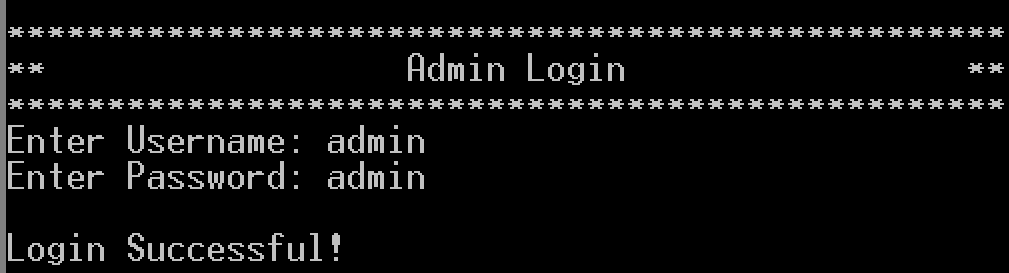
\includegraphics[scale=0.4]{Figures/login-success.png}
        \end{center}
        \caption{Login Page.}
     \end{figure}
    \begin{figure}[!htb]
\subsection{Main Menu}
Display main menu and prompt the use to make a choice.
        \begin{center}
         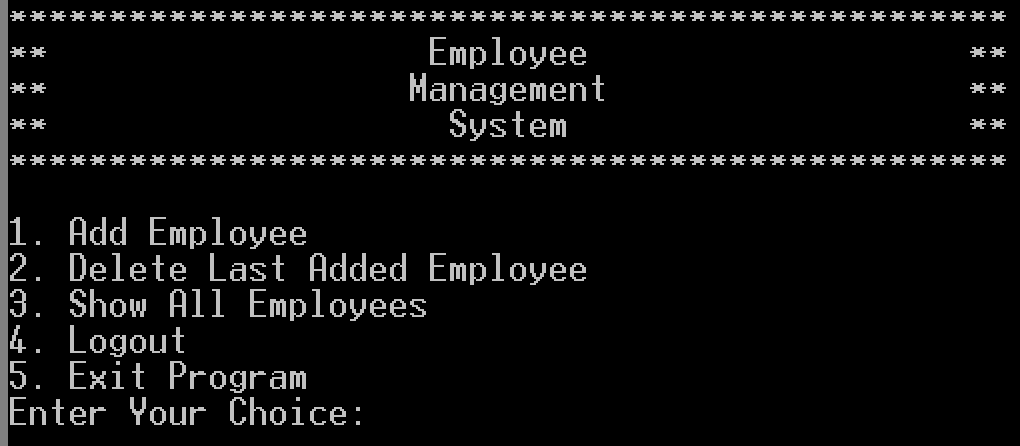
\includegraphics[scale=0.4]{Figures/main-menu.png}
        \end{center}
        \caption{Main Menu.}
     \end{figure}
    \begin{figure}[!htb]
\subsection{Add Employee}
Add employee name, email and phone.
        \begin{center}
         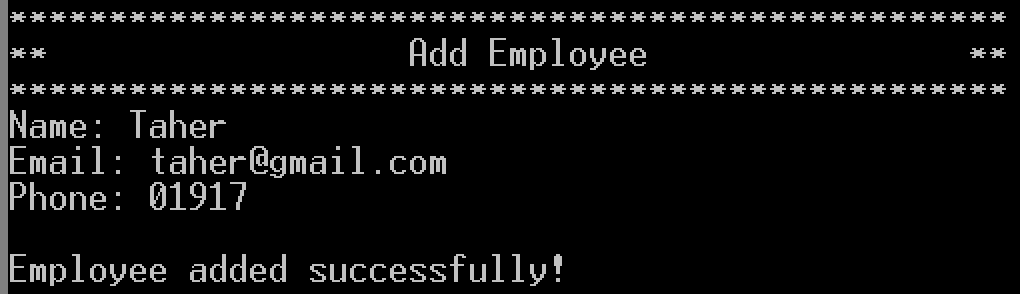
\includegraphics[scale=0.4]{Figures/add-emp.png}
        \end{center}
        \caption{Add Employee Page.}
     \end{figure}
    \begin{figure}[!htb]
\subsection{Delete Employee}
Delete the last added employee information.
        \begin{center}
         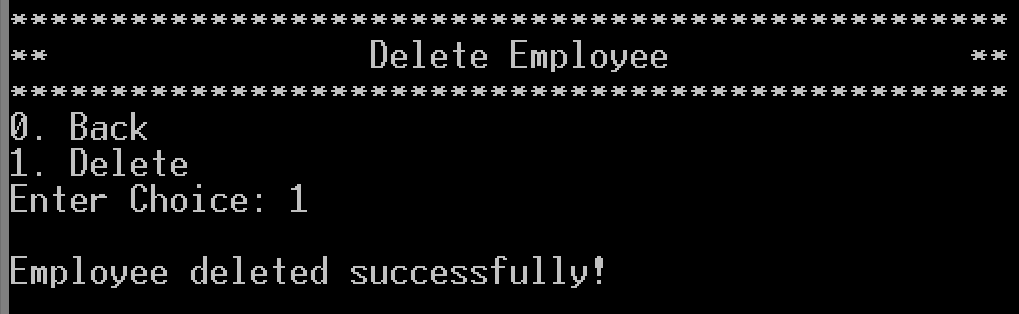
\includegraphics[scale=0.4]{Figures/delete-emp.png}
        \end{center}
        \caption{Delete Employee Page.}
     \end{figure}
    \begin{figure}[!htb]
\subsection{Show All Employee}
Show all existing employee information in a table format.
        \begin{center}
         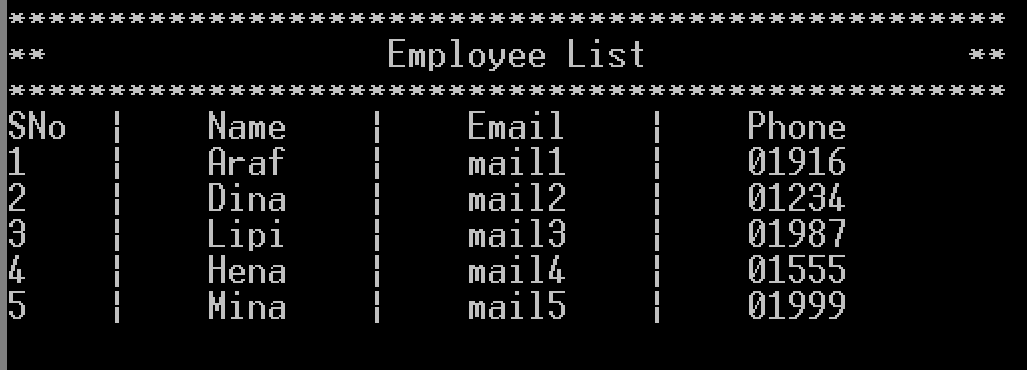
\includegraphics[scale=0.4]{Figures/show-all-emp.png}
        \end{center}
        \caption{Show All Employee Page.}
     \end{figure}


\begin{figure}
    \section{Results Overall Discussion}
This program successfully and efficiently handles the authentication procedure and basic managements such as, adding, deleting, and showing all employee information.
\end{figure}




% Chapter 3 ends here..... 




% Chapter 4 starts here..... 
\newpage
\chapter{Conclusion}

\section{Discussion}
\includecomment{Discuss the contents of this chapter and summarized the description of the work and the results and observation. Generally, it should be in one paragraph.}


In conclusion, the Employee Management System (EMS) is a simple and efficient tool for managing employee data. With features like authentication, adding and deleting employees, and viewing all employee information, it makes organizing employee records easy and secure.


\section{Limitations}
\includecomment{Discuss the limitations of the project. Limitations must be discussed, with the help of some critical analysis.}

Here are some potential limitations of this project:
\begin{itemize}
    \item The program can only handle a small amount of employee data because of the memory limitations.
    
    \item Employee information is lost when the program is closed since it doesn’t save data to a permanent storage.
    
    \item The system only includes basic functions like adding, deleting, and viewing employee information. It doesn’t have advanced options like searching or editing data.
\end{itemize}

\section{Scope of Future Work}
\includecomment{Discuss the future work of the project, that is your plans for more work and extension of your project.}

The scope of future work for this project could include:
\begin{itemize}

    \item Adding more advanced features like searching and updating employee information. 
    
    \item Integrating the system with payroll module to automate salary calculations and deductions based on employee data. 

     \item Implement some sorting functionalities based on some parameters.
\end{itemize}
\newline
These extensions can help employee management system to become more versatile, user-friendly, and robust.

% Chapter 5 ends here..... 

\section*{Reference}
 \begin{enumerate}
     \item \href{https://github.com/jacob5412/8086-Programs/blob/master/Expression/prompt_user_array%2Bdisplay.asm}{prompt-user-array+display - GitHub} 
     \item \href{https://github.com/topics/employee-management-system}{employee-management-system · GitHub Topics - GitHub} 
     \item \href{https://www.tutorialspoint.com/assembly_programming/assembly_loops.htm}{assembly-loops - TutorialsPoint}  
 \end{enumerate}

\end{comment}
\end{document}